\documentclass[12pt, letterpaper]{../assignment}
\usepackage{graphicx}
\usepackage{courier}
\usepackage{minted}
\usepackage{amsmath}
\usepackage{polynom}
\usepackage{commath}
\usepackage{amssymb}
\usepackage{amsfonts} 
\usepackage{color}
\usepackage{cancel}
\usepackage{enumitem}
\usepackage{graphicx}
\usepackage{multirow}
\usepackage{float}
\usepackage{bm}
\usepackage{tikz}
\usetikzlibrary{shapes,arrows}
\usepackage{booktabs}
\usetikzlibrary{patterns}

% Define Theme Colors
\definecolor{light-gray}{rgb}{0.2,0.2,0.2}
\definecolor{header-blue}{rgb}{0,0,0.7}
% \definecolor{header-blue}{rgb}{0.5137,0.8353,0.9176}
\definecolor{header-blue}{rgb}{0,0.8,0.95}
\definecolor{dark-gray}{rgb}{0.1,0.1,0.1}
\pagecolor{dark-gray}
\color{white}

\usemintedstyle{monokai}
\oddsidemargin = 0pt
\exercisesheet{Module 10}{Assignment}
\student{Austin Barrilleaux}
\university{\color{header-blue}Johns Hopkins University}
\school{\color{header-blue}Whiting School of Engineering}
\courselabel{EN 535.612}
\semester{Fall 2024}
\usepackage[backend=bibtex,style=numeric,sorting=none]{biblatex}
\bibliography{reference}

\definecolor{light-gray}{rgb}{0.2,0.2,0.2}
\setminted{bgcolor=light-gray,frame=lines,rulecolor=white}
\setlength{\parindent}{0pt}

\makeatletter
\patchcmd{\minted@colorbg}{\noindent}{\medskip\noindent}{}{}
\apptocmd{\endminted@colorbg}{\par\medskip}{}{}
\makeatother

\begin{document}

\subsection*{Problem 1: Multibody System}
\subsubsection*{The slider,
whose mass is $\bm{m_1}$ oscillates within the groove in the housing.
The moment of inertia of the housing about the axis of rotation is $\bm{I}$.
The spring restraining the slider is unstretched when $\bm{s = 0}$.
Derive differential equations for the distance $\bm{s}$ and spin angle $\bm{\phi}$ resulting from application of a torque $\bm{M(t)}$ to the shaft.}

\begin{figure}[H]
    \centering
    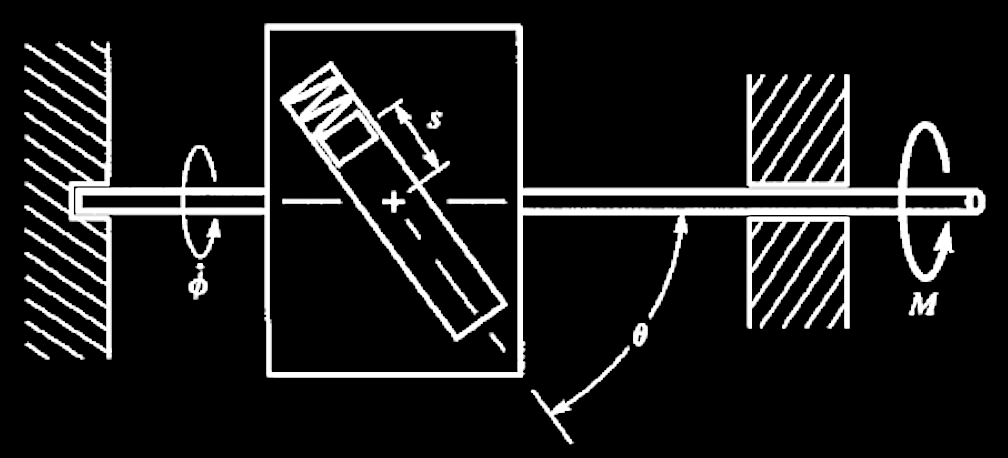
\includegraphics[scale=0.5,frame]{images/Problem_1.png}
\end{figure}


The following MATLAB function was used to solve this problem:

% \color{white}
\hspace*{6em}\inputminted[frame=leftline,fontsize=\footnotesize,lastline=32]{matlab}
{./matlab/Problem_1.m}
% \color{black} 


\subsection*{Problem 2: Nonholonomic System}
\subsubsection*{
A known couple $\bm{M(t)}$ is applied to the upper bar.
Force $\bm{F}$, which is applied perpendicularly to the lower bar,
acts to make the velocity of end $\bm{C}$ always be parallel to the line from joint $\bm{A}$ to end $\bm{B}$.
The bars have equal mass $\bm{m}$,
and the system lies in the vertical plane.
Use the method of Lagrange multipliers to derive the equations of motion.}

\begin{figure}[H]
    \centering
    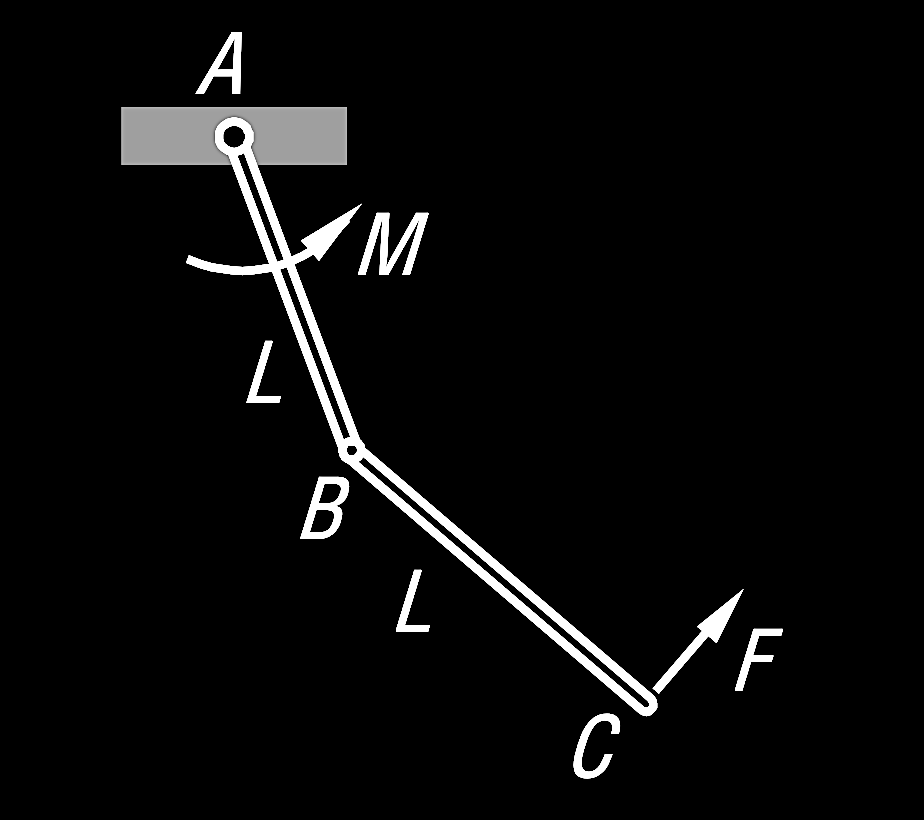
\includegraphics[scale=0.35,frame]{images/Problem_2.png}
\end{figure}


% % \color{white}
% \hspace*{6em}\inputminted[frame=leftline,fontsize=\footnotesize]{matlab}
% {./matlab/Q6_8.m}
% % \color{black} 

% \begin{figure}[H]
%     \centering
%     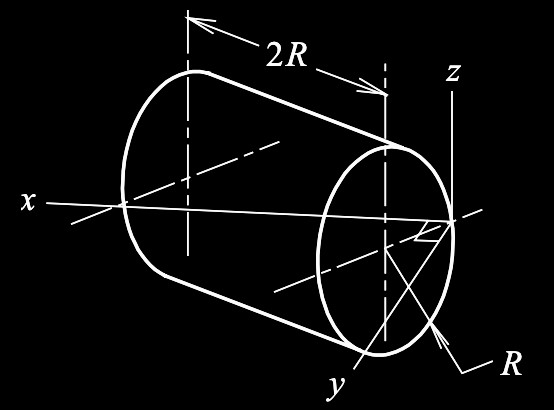
\includegraphics[scale=0.7,frame]{images/Q5_13.png}
% \end{figure}




\end{document}

